\documentclass[11pt]{article}

\usepackage[margin=1in]{geometry}
\usepackage{graphicx}
\usepackage{booktabs}
\usepackage{array}
\usepackage{amsmath}
\usepackage{amssymb}
\usepackage{hyperref}
\usepackage{xcolor}
\usepackage{enumitem}

\graphicspath{{./}{reports/}}

\title{LangGraph RAG System Report}
\author{Product Documentation RAG Project}
\date{July 1, 2026}

\begin{document}

\maketitle

\begin{abstract}
This report summarizes a corpus-first Retrieval Augmented Generation (RAG) system built
with LangGraph over a product documentation snapshot. From 1,218 raw HTML files, the
pipeline kept 729 documents and indexed 1,494 chunks after extraction, filtering, and
deduplication. On a 48-item evaluation set, the corpus-only configuration achieved
MRR 0.745, Recall@10 0.9208, Hit@10 0.975, faithfulness 0.9712, answer relevance
0.9963, citation presence 0.975, abstention recall 1.000, and zero false abstentions,
with mean latency near 2.15 seconds. The web-augmented run triggered web search on
4.2\% of queries but added no final web context and did not improve retrieval or
citation metrics, so the recommended operating mode is corpus-only until a stronger
freshness provider or targeted web policy is added. The suggested next solution is to
keep the current hybrid lexical+dense retrieval and Qwen reranking pattern, but scale it
with an approximate-nearest-neighbor index for million-document corpora and add
label-agnostic monitoring through hierarchical weak labels, citation coverage, and
query/answer stability checks.
\end{abstract}

\tableofcontents
\newpage

\section{Project Overview}

The goal is to build a cited question-answering assistant for product and support
documentation. The assistant should answer from retrieved evidence, expose citations, and
decline when the available context is insufficient. The implementation is modular:
configuration selects retrievers, rerankers, model endpoints, guards, and optional web
augmentation without changing graph code.

The system uses two runtime layers. The orchestration layer is a lightweight Python
environment that runs LangGraph, ingestion, retrieval, evaluation, and the UI. Model
inference is served separately through OpenAI-compatible vLLM endpoints. This separation
keeps the RAG code portable while allowing the model-serving layer to be tuned
independently for GPU memory and throughput.

\section{Corpus Preparation}

The raw corpus contains 1,218 HTML files. After extraction, filtering, and deduplication,
729 documents were kept for indexing. The resulting index contains 1,494 chunks. Chunking
is heading-aware, with a target of 512 tokens and 64-token overlap, so context units retain
section structure while remaining short enough for reranking and generation.

\begin{table}[h]
\centering
\begin{tabular}{lr}
\toprule
Corpus statistic & Count \\
\midrule
Raw HTML files & 1,218 \\
Kept documents & 729 \\
Indexed chunks & 1,494 \\
\bottomrule
\end{tabular}
\caption{Corpus size after cleaning and chunking.}
\end{table}

\begin{table}[h]
\centering
\begin{tabular}{lr}
\toprule
Drop reason & Count \\
\midrule
Empty after extraction & 238 \\
Duplicate content & 184 \\
Dropped page type & 64 \\
Too small & 2 \\
Non-English & 1 \\
\bottomrule
\end{tabular}
\caption{Dropped document categories during corpus cleaning.}
\end{table}

``Empty after extraction'' does not mean that the raw HTML files were empty. It means that
after scripts, navigation, forms, and template content were removed, fewer than 200 useful
text characters remained. Many such files are client-side-rendered support pages where the
article body is absent from the static crawl. A JavaScript-rendered recrawl would be needed
to recover those pages.

\section{Architecture and System Graph}

Figure~\ref{fig:system-graph} shows the runtime architecture. The graph can be regenerated
with:

\begin{verbatim}
python -m langgraph_rag.obs.render_graphs
\end{verbatim}

\begin{figure}[h]
\centering
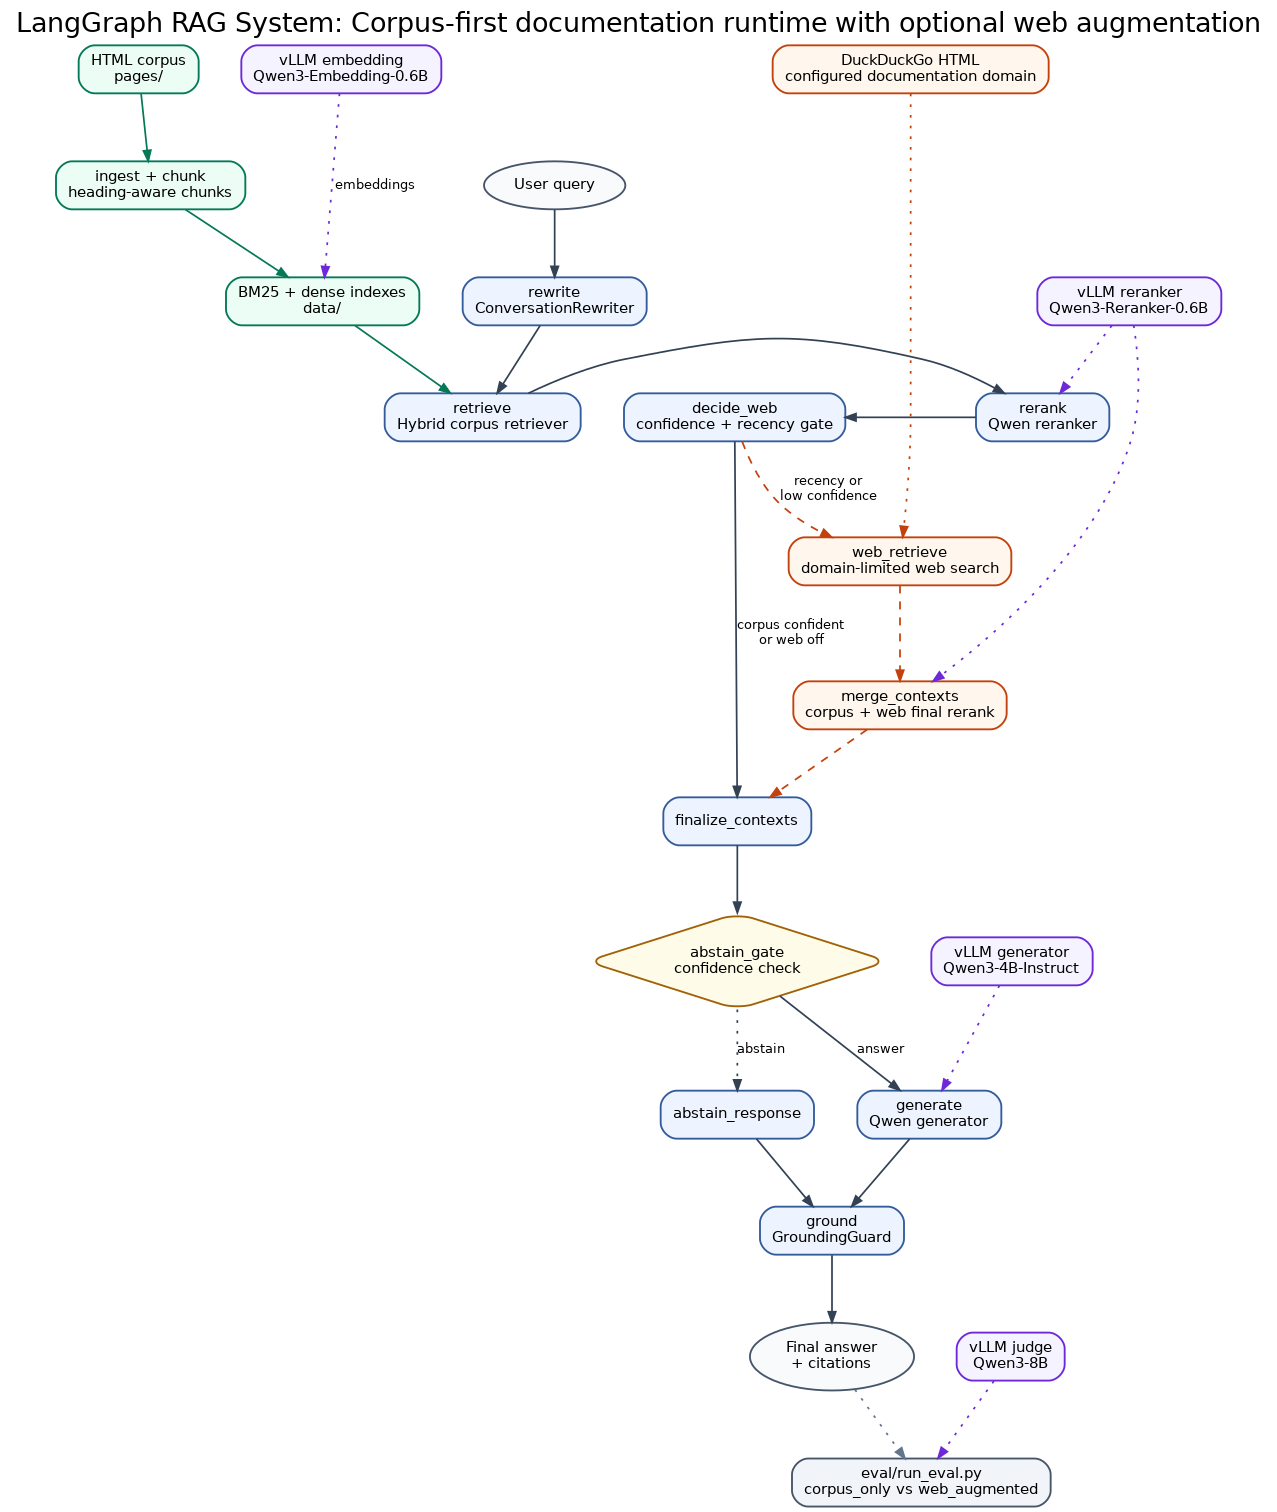
\includegraphics[width=0.95\textwidth]{graphs/system_graph.png}
\caption{LangGraph RAG system architecture.}
\label{fig:system-graph}
\end{figure}

The graph has four main sections:

\begin{enumerate}[leftmargin=*]
  \item \textbf{Offline corpus path.} Raw pages are cleaned, deduplicated, chunked, and
  indexed into dense and lexical stores. This path is run during corpus refreshes rather
  than at query time.
  \item \textbf{Runtime answer path.} A user query may be rewritten, then passed through
  hybrid retrieval, reranking, optional web routing, abstention, generation, and grounding.
  \item \textbf{Model services.} Embedding, reranking, generation, and judging run as
  separate vLLM services. The graph communicates with them through HTTP endpoints.
  \item \textbf{Evaluation and observability.} Evaluation scripts compare corpus-only and
  web-augmented conditions, while the UI and reports expose traces, citations, and user
  feedback.
\end{enumerate}

\section{Model Choices}

The system uses specialized Qwen models for different stages rather than one model for all
work. This reduces cost, makes latency easier to control, and lets each component use a
model suited to its role.

\begin{table}[h]
\centering
\small
\begin{tabular}{p{0.18\textwidth}p{0.27\textwidth}p{0.46\textwidth}}
\toprule
Role & Model & Reason for use \\
\midrule
Embedding &
\texttt{Qwen3-Embedding-0.6B} &
Compact embedding model with 1024-dimensional vectors. It is efficient enough for repeated
query embedding and index construction while preserving semantic matching beyond exact
keyword overlap. \\
\addlinespace
Reranking &
\texttt{Qwen3-Reranker-0.6B} &
Cross-encoder relevance scoring improves the final context set after broad hybrid
retrieval. The small reranker is fast enough to apply to the top retrieval candidates
before generation. \\
\addlinespace
Generation &
\texttt{Qwen3-4B-Instruct-2507} &
Instruction-tuned model used for cited answers. It is a practical quality/latency tradeoff
for local serving and can follow prompts requiring abstention and source-grounded output. \\
\addlinespace
Judge / grounding &
\texttt{Qwen3-8B} &
Larger model used for evaluation and claim support checks. It is intentionally different
from the generator to reduce self-evaluation bias during faithfulness and grounding checks. \\
\bottomrule
\end{tabular}
\caption{Configured model services and their roles.}
\end{table}

All model names and endpoints are configured in \path{langgraph_rag/config/settings.yaml}.
The code calls these services through OpenAI-compatible APIs, so swapping a model is a
configuration change rather than a code change.

\section{Retrieval and Generation Pipeline}

\subsection{Hybrid Retrieval}

Retrieval uses both dense search and BM25. Dense search embeds the query and compares it
with precomputed chunk embeddings, which helps with semantic matches and paraphrases.
BM25 protects exact terms such as product names, feature names, version strings, and
technical abbreviations. The two ranked lists are fused with Reciprocal Rank Fusion (RRF),
which is rank-based and avoids comparing incompatible score scales.

The first retrieval stage returns 20 candidates. This deliberately over-fetches so the
reranker has enough material to select a stronger final context set.

\subsection{Reranking and Context Selection}

The reranker scores query--chunk pairs and keeps the top 5 final contexts for generation.
The highest rerank score is stored as \texttt{top\_score}. It is a retrieval-confidence
signal, not a ground-truth correctness score. The graph uses it for abstention and, when
enabled, for web fallback decisions.

\subsection{Answer Generation and Citations}

The generator receives the query, recent chat history, and the final context set. It is
prompted to answer only from the provided sources and to include inline citations. The
system stores citations as structured records containing title, URL, and chunk id, which
makes answers inspectable in the UI and measurable during evaluation.

\subsection{Abstention and Grounding}

The abstention guard prevents answers when evidence is too weak or unavailable. After an
answer is produced, the grounding guard splits it into claims and checks whether each claim
is supported by the retrieved context. Groundedness is therefore a source-support signal,
not a guarantee of real-world truth.

\subsection{Optional Web Augmentation}

Web augmentation is not the default path. When enabled, a confidence and recency gate can
trigger domain-limited web search for freshness-sensitive queries. The current provider
triggered on a small number of questions but produced no final web context in the latest
evaluation, so corpus-only remains the recommended mode.

\section{Evaluation Results}

The evaluation set contains 48 items: 40 synthetic items and 8 curated items. Metrics cover
retrieval quality, generation quality, citation behavior, abstention, web usage, and
latency.

\begin{table}[h]
\centering
\small
\begin{tabular}{lrrr}
\toprule
Metric & Corpus-only & Web-augmented & Delta \\
\midrule
MRR & 0.745 & 0.745 & 0.000 \\
Hit@10 & 0.975 & 0.975 & 0.000 \\
Faithfulness & 0.9712 & 0.9700 & -0.0012 \\
Answer relevance & 0.9963 & 0.9925 & -0.0038 \\
Has citation rate & 0.975 & 0.975 & 0.000 \\
Gold doc cited rate & 0.647 & 0.647 & 0.000 \\
Abstain recall & 1.000 & 1.000 & 0.000 \\
False abstain rate & 0.000 & 0.000 & 0.000 \\
Mean latency (ms) & 2,152 & 2,119 & -33 \\
P90 latency (ms) & 4,616 & 4,565 & -51 \\
Web trigger rate & 0.000 & 0.042 & 0.042 \\
Final web context rate & 0.000 & 0.000 & 0.000 \\
\bottomrule
\end{tabular}
\caption{Latest corpus-only vs. web-augmented evaluation summary.}
\end{table}

Retrieval is strong at broader cutoffs: hit@10 is 0.975 and recall@10 is 0.9208 in both
conditions. Recall@1 is lower at 0.35, which means the correct source is often present in
the candidate set but not always ranked first. This supports keeping the reranker and
generator context window rather than relying on top-1 retrieval alone.

Generation quality is high in both conditions, with corpus-only faithfulness at 0.9712 and
answer relevance at 0.9963. Citation coverage is also high, with has-citation rate at
0.975. The stricter gold-document citation rate is 0.647; this metric penalizes answers
that cite a related source rather than the exact synthetic gold document.

Abstention behavior is strong in the current evaluation: unanswerable recall is 1.0 and
false abstention on answerable items is 0.0. Latency is acceptable for a local multi-model
pipeline, with mean latency around 2.1 seconds and p90 around 4.6 seconds in the latest
reports.

\section{Future Work}

\subsection{Scaling Retrieval to Millions of Documents}

The current dense retrieval path is appropriate for a prototype-sized corpus, but a
million-document deployment needs a different retrieval architecture. The first step is to
move from simple local dense arrays to approximate nearest-neighbor indexing such as HNSW,
IVF, or product-quantized FAISS indexes, or to a distributed vector database. Metadata
filters should run before expensive vector search so that product, language, date, and
document-type constraints shrink the candidate set early.

The second step is incremental indexing. Large documentation systems change continuously,
so index versioning, document hashing, and chunk-level updates are preferable to full
rebuilds. Query embedding caches and retrieval caches can reduce repeated work, while
batch reranking can improve GPU utilization. A practical large-scale design would keep the
current two-stage pattern: broad lexical+dense retrieval over millions of chunks, followed
by cross-encoder reranking over only a small candidate pool.

\subsection{Label-Agnostic Evaluation Without Labels or Judge Models}

The current evaluation uses synthetic labels, curated examples, and an LLM judge. A future
system should also support label-agnostic evaluation, where no ground-truth labels and no
LLM-as-judge are required. This can be done with deterministic and behavioral signals:
retrieval stability under paraphrases, agreement between dense and lexical retrieval,
answer stability under query rewrites, citation coverage, source URL diversity, abstention
consistency, and sensitivity tests where removing the top context should reduce confidence.

Another direction is source-attribution auditing without a judge model. The system can
measure whether cited chunks contain the named entities, numbers, dates, and short quoted
phrases used in the answer. It can also track drift over time: sudden changes in score
distributions, citation rates, abstention rates, or latency can flag regressions even when
labels are unavailable. Human feedback from the UI can then be sampled for review and
converted into future labeled tests only when needed.

\section{Reproducibility}

The main commands are:

\begin{verbatim}
# Run tests
python -m pytest -q

# Run corpus-only evaluation
python -m langgraph_rag.eval.run_eval --condition corpus_only

# Run web-augmented evaluation
python -m langgraph_rag.eval.run_eval --condition web_augmented

# Regenerate graph artifacts
python -m langgraph_rag.obs.render_graphs
\end{verbatim}

Evaluation reports are written under \path{reports/}. Graph artifacts are written under
\path{reports/graphs/}. The UI stores chat sessions under \path{data/ui/sessions/} and
feedback records under \path{data/ui/feedback.jsonl}.

\appendix

\section{Chatbot UI Features}

The project includes a local Streamlit chatbot UI. It can be started with:

\begin{verbatim}
streamlit run langgraph_rag/app/streamlit_app.py \
  --server.port 8501 --server.address 0.0.0.0 --server.headless true
\end{verbatim}

The UI supports:

\begin{itemize}[leftmargin=*]
  \item multi-turn chat with saved local sessions;
  \item cited answers with clickable source URLs;
  \item expandable retrieved-context inspection;
  \item trace visibility, including top score, retrieval latency, rerank latency,
        generation latency, web latency, and total latency;
  \item friendly error handling when backend model services are unavailable;
  \item per-answer positive or negative feedback with optional comments;
  \item an Admin view for evaluation reports, A/B deltas, sample answers, feedback review,
        and source artifact paths.
\end{itemize}

Saved sessions are local JSON files, and feedback is append-only JSONL. No external UI
logging service is required.

\section{Hierarchical Weak-Label Evaluation for Large-Scale RAG Retrieval}
\label{sec:hierarchical-weak-label-eval}

\subsection{Problem: RAG Evaluation Without Exhaustive Ground-Truth Labels}

Evaluating retrieval-augmented generation (RAG) systems at large scale is difficult because exhaustive query--document relevance labels are usually unavailable. In a small benchmark, one may manually annotate which documents are relevant to each query and then compute standard retrieval metrics such as Recall@$k$, MRR, or nDCG. However, this strategy does not scale to production retrieval settings where the database may contain millions or billions of documents and the query distribution changes continuously.

This creates a fundamental evaluation gap. For a query $q$, the system retrieves a ranked list of documents
\[
R(q) = [d_1, d_2, \ldots, d_k],
\]
but we often do not know the true relevant set
\[
G(q) = \{d^\star_1, d^\star_2, \ldots\}.
\]
Without $G(q)$, standard supervised retrieval metrics become unreliable or impossible to compute directly. This is especially problematic for RAG, because retrieval errors propagate into generation errors. If the retriever fails to surface the correct evidence, the generator may hallucinate, abstain unnecessarily, or produce an answer that is topically related but unsupported.

A second issue is that binary relevance labels are often too rigid for large-scale semantic retrieval. A retrieved document may not exactly answer the query, but it may belong to the correct product family, topic, or subdomain. For example, for a query about 3D modeling limits in a lightweight design tool, a document about that tool's feature limitations is more relevant than a general design-tool overview, which is still more relevant than a document about an unrelated media-production suite. Therefore, we need an evaluation signal that can express graded semantic closeness rather than only binary relevance.

\subsection{Proposed Solution: Hierarchical Semantic Clustering as Weak Ground Truth}

We propose to construct a large-scale hierarchical semantic clustering of the document corpus and use the resulting hierarchy as a weak labeling structure for RAG evaluation. Instead of requiring manually labeled relevant documents for every query, we assign documents, queries, retrieved contexts, and generated answer claims into a shared multi-resolution semantic tree.

At the lowest level, documents are grouped into fine-grained micro-clusters. These micro-clusters are then recursively clustered into coarser semantic groups. For a billion-document corpus, a possible hierarchy is:
\[
\begin{aligned}
10^9\ \text{documents}
&\rightarrow 10^7\ \text{micro-clusters} \\
&\rightarrow 10^5\ \text{mid-level clusters} \\
&\rightarrow 10^3\ \text{broad clusters} \\
&\rightarrow 10\ \text{root domains}.
\end{aligned}
\]
This hierarchy creates a multi-resolution semantic map of the corpus. Each document has a path from a root cluster to a fine-grained leaf cluster:
\[
\pi(d) = [c^{(0)}(d), c^{(1)}(d), \ldots, c^{(L)}(d)],
\]
where $c^{(0)}$ is the root-level cluster and $c^{(L)}$ is the finest cluster.

The motivation for this design is related to recent work on hierarchical document clustering with Matryoshka-style embeddings, where different embedding truncation levels capture different semantic granularities. This suggests a natural direction for RAG evaluation: use coarse embedding views for broad domain agreement and high-dimensional views for fine-grained evidence matching.

\subsection{Hierarchy Construction}

The hierarchy can be constructed in an offline stage. First, every document or chunk $d_i$ is encoded into an embedding vector:
\[
z_i = f_{\theta}(d_i).
\]
For large collections, exact all-pairs clustering is infeasible. Therefore, we use scalable approximate methods such as approximate nearest-neighbor search, recursive balanced $k$-means, graph-based clustering, or approximate agglomerative clustering.

At the first level, documents are grouped into fine-grained clusters:
\[
\mathcal{C}^{(L)} =
\{C^{(L)}_1, C^{(L)}_2, \ldots, C^{(L)}_{M_L}\}.
\]
Each fine cluster is represented by a centroid:
\[
\mu_j^{(L)} =
\frac{1}{|C^{(L)}_j|}
\sum_{d_i \in C^{(L)}_j} f_{\theta}(d_i).
\]
Then the centroids are clustered again to form the next coarser level:
\[
\mathcal{C}^{(L-1)} =
\text{Cluster}\left(\{\mu_j^{(L)}\}_{j=1}^{M_L}\right).
\]
This process repeats until a small number of root clusters is obtained.

For interpretability, each cluster should store:
\[
\begin{aligned}
\text{cluster node} =
&\{\text{centroid}, \text{representative documents}, \\
&\text{keywords/entities}, \text{LLM-generated label}, \\
&\text{parent id}, \text{children ids}\}.
\end{aligned}
\]
For example, a cluster path may look like:
\[
\begin{aligned}
\text{Product documentation}
&\rightarrow \text{Design tools} \\
&\rightarrow \text{Lightweight design-tool capabilities} \\
&\rightarrow \text{3D modeling limitations}.
\end{aligned}
\]

\subsection{Query and Retrieval Evaluation Using Tree Distance}

Given a user query $q$, we embed it and assign it to the hierarchy:
\[
\pi(q) = [c^{(0)}(q), c^{(1)}(q), \ldots, c^{(L)}(q)].
\]
The retrieved documents $R(q) = [d_1, \ldots, d_k]$ are already assigned to cluster paths $\pi(d_i)$. We can then evaluate retrieval quality using hierarchical agreement rather than exact ground-truth relevance.

We define the common-prefix depth between a query and document as:
\[
\text{CP}(q, d) =
\max_{\ell} \left\{ \ell : c^{(j)}(q) = c^{(j)}(d),\ \forall j \leq \ell \right\}.
\]
A document that shares the same fine-grained cluster with the query receives the highest score, while a document that only shares a broad root cluster receives a lower score. A simple hierarchical relevance score is:
\[
s_{\text{hier}}(q,d) = \frac{\text{CP}(q,d)}{L}.
\]
Alternatively, we can use manually chosen level weights:
\[
s_{\text{hier}}(q,d) =
\begin{cases}
1.0, & \text{same fine cluster},\\
0.7, & \text{same parent cluster},\\
0.4, & \text{same grandparent cluster},\\
0.1, & \text{same root domain},\\
0.0, & \text{different root domain}.
\end{cases}
\]

This gives a weak relevance score without requiring manually annotated query--document labels. We can then compute weak-label versions of retrieval metrics:
\[
\text{HierRecall@}k =
\frac{1}{k} \sum_{i=1}^{k} \mathbb{I}\left[s_{\text{hier}}(q,d_i) \geq \tau \right],
\]
where $\tau$ is a relevance threshold at the desired semantic granularity. We can also define a hierarchical DCG:
\[
\text{H-DCG@}k =
\sum_{i=1}^{k} \frac{s_{\text{hier}}(q,d_i)}{\log_2(i+1)}.
\]
This measures whether highly ranked documents are semantically close to the query in the document hierarchy.

\subsection{Cluster-Aware Query Decomposition}

Complex queries often require evidence from multiple semantic regions. For example:
\[
q = \text{``Compare Tool A and Tool B for 3D modeling and collaboration.''}
\]
A single cluster assignment may be insufficient because the query combines multiple products and multiple aspects. Therefore, we decompose complex queries into subqueries:
\[
q \rightarrow \{q_1, q_2, \ldots, q_m\}.
\]
Each subquery should be answerable from one focused semantic cluster:
\[
\begin{aligned}
q_1 &= \text{``What 3D modeling features does Tool A provide?''} \\
q_2 &= \text{``What 3D modeling features does Tool B provide?''} \\
q_3 &= \text{``What collaboration features are described for Tool A and Tool B?''}
\end{aligned}
\]
Each subquery is independently assigned to the hierarchy and retrieves evidence from its corresponding cluster region. The final answer is generated by merging the evidence sets:
\[
E(q) = \bigcup_{j=1}^{m} R(q_j).
\]
This improves both retrieval coverage and evaluation. Instead of asking whether all retrieved documents match one query cluster, we evaluate whether each subquery retrieves evidence from its expected cluster.

\subsection{Answer Claim Evaluation Using the Same Hierarchy}

The hierarchy can also support generation evaluation. After the RAG system generates an answer $a$, we split it into atomic claims:
\[
a \rightarrow \{\gamma_1, \gamma_2, \ldots, \gamma_n\}.
\]
Each claim $\gamma_i$ is embedded and assigned to the hierarchy. We then check whether its cluster is covered by the retrieved evidence clusters:
\[
\text{covered}(\gamma_i, E) =
\mathbb{I}\left[
\exists d \in E \text{ such that } s_{\text{hier}}(\gamma_i,d) \geq \tau_c
\right].
\]
The cluster-based claim support score is:
\[
\text{ClusterClaimSupport}(a,E) =
\frac{1}{n}\sum_{i=1}^{n}\text{covered}(\gamma_i,E).
\]
This is not a replacement for factual entailment, because two claims may be in the same semantic cluster but contradict each other. However, it is a scalable weak signal for detecting unsupported topic drift. If an answer contains claims whose clusters are absent from the retrieved evidence, the answer is suspicious and should be flagged for a stronger LLM-based grounding check.

\subsection{Use in RAG Monitoring}

The proposed hierarchy gives several useful no-ground-truth monitoring signals:
\[
\begin{gathered}
\text{QueryClusterConfidence}, \quad
\text{RetrievalClusterAgreement}, \quad
\text{HierarchicalDCG}, \\
\text{ClusterClaimSupport}, \quad
\text{OutOfDomainScore}.
\end{gathered}
\]
These signals can be logged for every query. For example, a low query-cluster confidence indicates that the query may be out of domain. Low retrieval-cluster agreement indicates that the retriever may have returned topically irrelevant evidence. Low claim-support indicates that the generator may have introduced unsupported claims. These metrics do not require manual labels for every query and therefore can be applied continuously at production scale.

\subsection{Limitations and Validation}

The proposed hierarchy provides weak labels, not absolute truth. Cluster membership measures semantic proximity, but it does not guarantee factual support, polarity, temporal correctness, or entailment. For example, two documents may belong to the same feature-limitations cluster while making different claims about availability. Therefore, hierarchical cluster evaluation should be used as a scalable diagnostic layer, not as the only evaluation method.

To validate the weak-label evaluator, we should manually annotate a small but diverse set of queries and compare human judgments with the hierarchy-based scores. This allows us to measure whether tree-distance scores correlate with human relevance judgments. In addition, cluster-based claim support should be combined with LLM-based claim-level grounding checks for higher precision on faithfulness evaluation.

Overall, the proposed method reframes the absence of ground-truth labels as a weak-supervision problem. By constructing a hierarchical semantic map of the document corpus, we can estimate retrieval quality and answer support using tree-distance and cluster-coverage metrics. This enables large-scale RAG evaluation in settings where exhaustive relevance labeling is infeasible.

\end{document}
